\chapter{Validation of Embedded Systems Approach}

Before designing the embedded CMS, the sensors were tested on the CML for comparison to each other and, where possible, to a reference sensor on the existing system.
This is important as the CML provides very different conditions to the laboratory setting.
In addition to gaining more information about the sensors, these tests will also allow an evaluation of the relative merits of MCSA and vibration analysis for condition monitoring of the CML.
These tests also provided an environment to improve the design of embedded CMS hardware and software.
\par

\section{Vibration Analysis}

\subsection{Sensor Comparison}

\begin{figure}
    \centering
    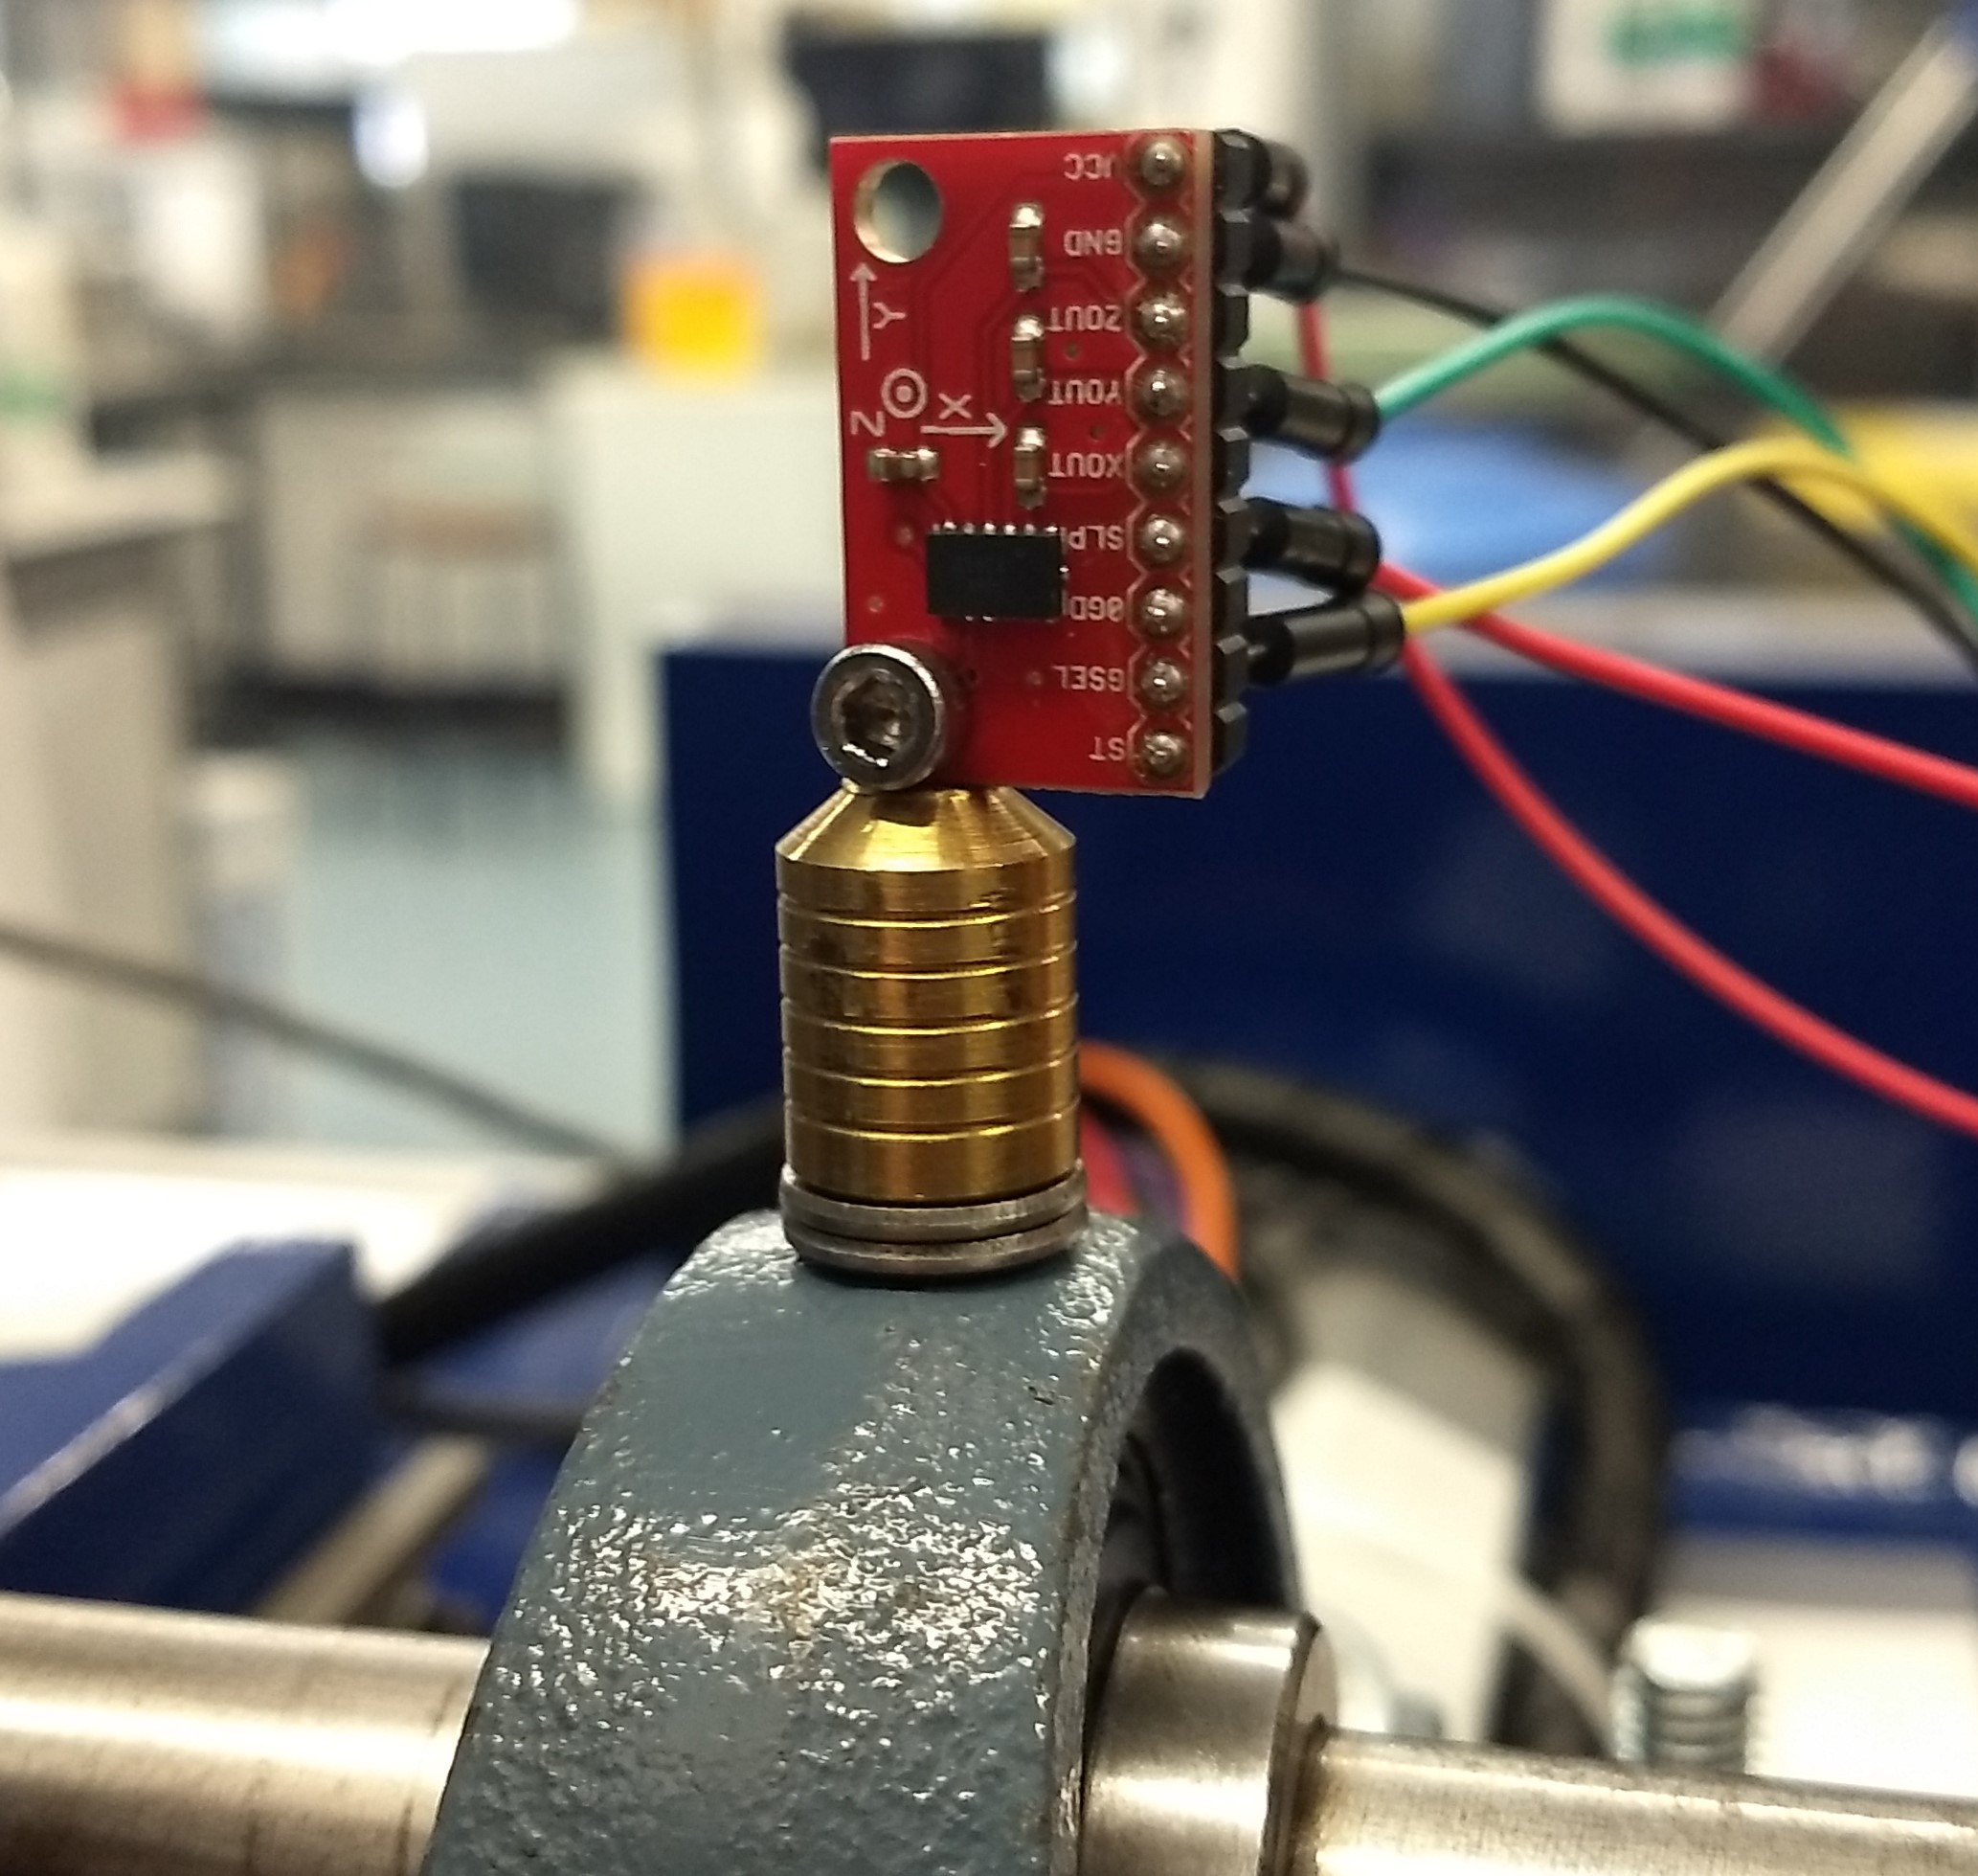
\includegraphics[width=0.5\linewidth]{Mechanical_Fixing3.jpg}
    \caption{Mechanical fixing for MEMS sensors on bearing}
    \label{fig:Mechanical_Fixing}
\end{figure}

Following the work in section (3??), vibration analysis is a promising candidate for condition monitoring of the CML.
It is also clear that there are significant differences in how the available MEMS sensors perform, particularly at frequencies in the kHz range.
Testing on the CML allows for an informed decision about which sensor to use in the final design.
\par

The CML was placed into a healthy condition.
As noted, the exact condition of the CML is hard to control, so to provide a baseline for comparison of the sensors, measurements were also taken from the existing accelerometer, referred to as \textit{ref}.
Bearing 2 was chosen due to its ability to give clear information about machine condition.
Five samples were taken with each sensor.
For the MEMS sensors, the frequency spectrum was calculated on board and transferred to a computer.
The \textit{ref} sensor values were stored on the CML computer and processed offline.
Average frequency spectrums across the samples were calculated.
The \textit{ref} sensor was sampled at 5 kHz.
To ensure that all frequency components measured by the \textit{ref} sensor were included, the MEMS sensors were sampled at 8192 Hz.
\par

The MEMS sensors were mounted with a mechanical screw fixing, which allowed the evaluation boards to be attached in a similar manner to the banana plug used previously (Fig \ref{fig:Mechanical_Fixing}).
Two washers were used to prevent the end of the bolt from pressing on the bearing casing and influencing the vibrations.
Therefore, the MEMS and \textit{ref} sensors were all mounted in the same hole, diminishing the effect of mounting on the vibration signal.
\par

\begin{figure}
    \centering
    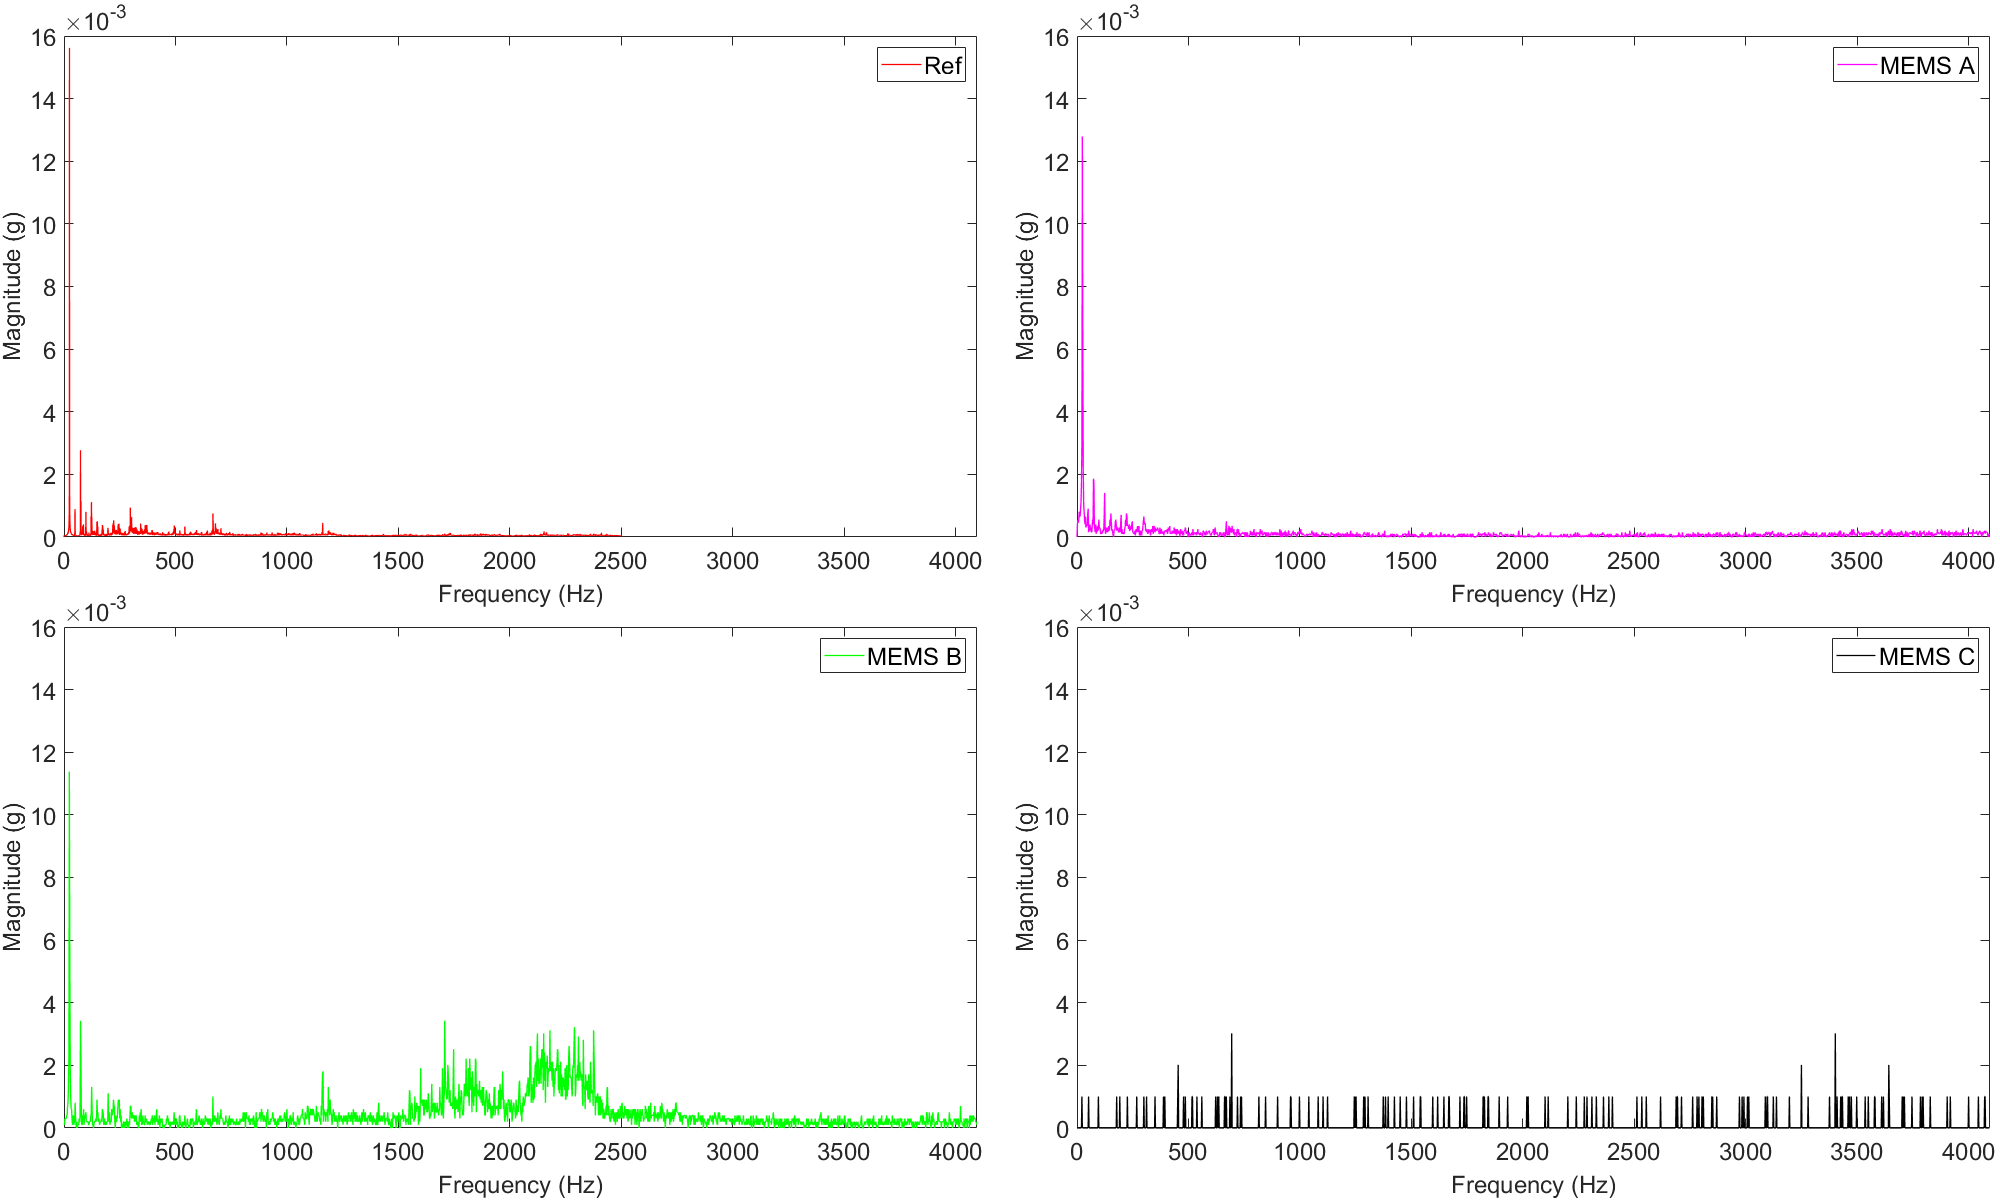
\includegraphics[width=\linewidth]{SensorTest_Comparison.png}
    \caption{Comparison of \textit{ref} and MEMS sensors}
    \label{fig:SensorTest_Comparison}
\end{figure}

The averaged frequency spectrums show good agreement with \textit{ref} for MEMS A and B at the lower frequencies, while MEMS C clearly struggles to detect the vibration signals (Fig \ref{fig:SensorTest_Comparison}).
This is simply a result of the vibration level being too low for the sensor to discern signals from the motor from background noise.
While MEMS C had been found to be a good candidate, the measurement range is too large for the signals from the CML and the measurement resolution with the ADC setup.
This provides a clear reminder of the importance of adapting CMSs to the specific implementation.
Further, there is a large amount of noise in the spectrum of MEMS B from 1500 to 2500 Hz.
The frequency response curve for this sensor shows a rise in magnitudes for frequencies in this range before a steep decline \cite{ADXL354}.
However, this level of noise was not observed during initial sensor testing.
Processing of the data found that some of this noise could be removed with a low pass filter at around 1 kHz, however this would remove the possibility of identifying frequency components at higher frequencies.
MEMS A better characterises the frequency spectrum of the bearing, with a magnitude closer to \textit{ref} at the rotor frequency and a less noisy signal overall.
\par

Therefore, MEMS A is selected as the accelerometer for the embedded CMS and will undergo further testing.


\subsection{Condition Monitoring}

To inform the final system, the MEMS A and ref sensors were tested on the CML in different conditions.
Again, healthy, bent and faulty bearings are the conditions.
This would help identify differences in the signals and the ability of MEMS A to differentiate between the conditions.
\par

Five samples were taken in each condition, with the sensors being tested one after the other without interfering with the CML to prevent small differences in condition.
In addition to the frequency spectrum, the time data was also plotted against the ISO bearing fault severity chart \cite{ISO13373-3}.
The remaining parameters are the same as the previous test.
\par

It is expected that there will be some small differences in the data from the sensors.
The \textit{ref} sensor collects more samples and therefore has a higher resolution, as well as a higher frequency range.
This should lead to a more accurate frequency spectrum.
However, it was found that the statistics of the spectrum lead to clearly identifiable groups when plotted; this is expected also in the data from MEMS A.
\par

Samples of the time data collected are shown in Fig \ref{fig:SensorTest_T}.
There is good agreement between the sensors in terms of magnitude and overall signal shape.
The bent condition is clearly identifiable by a large amount of noise.
Signal magnitude increases significantly for the \textit{ref} sensor but not for MEMS A.
Differences between the healthy and faulty bearing state are much harder to identify in the time domain.
Nevertheless, these results are promising.
\par

\begin{figure}
    \centering
    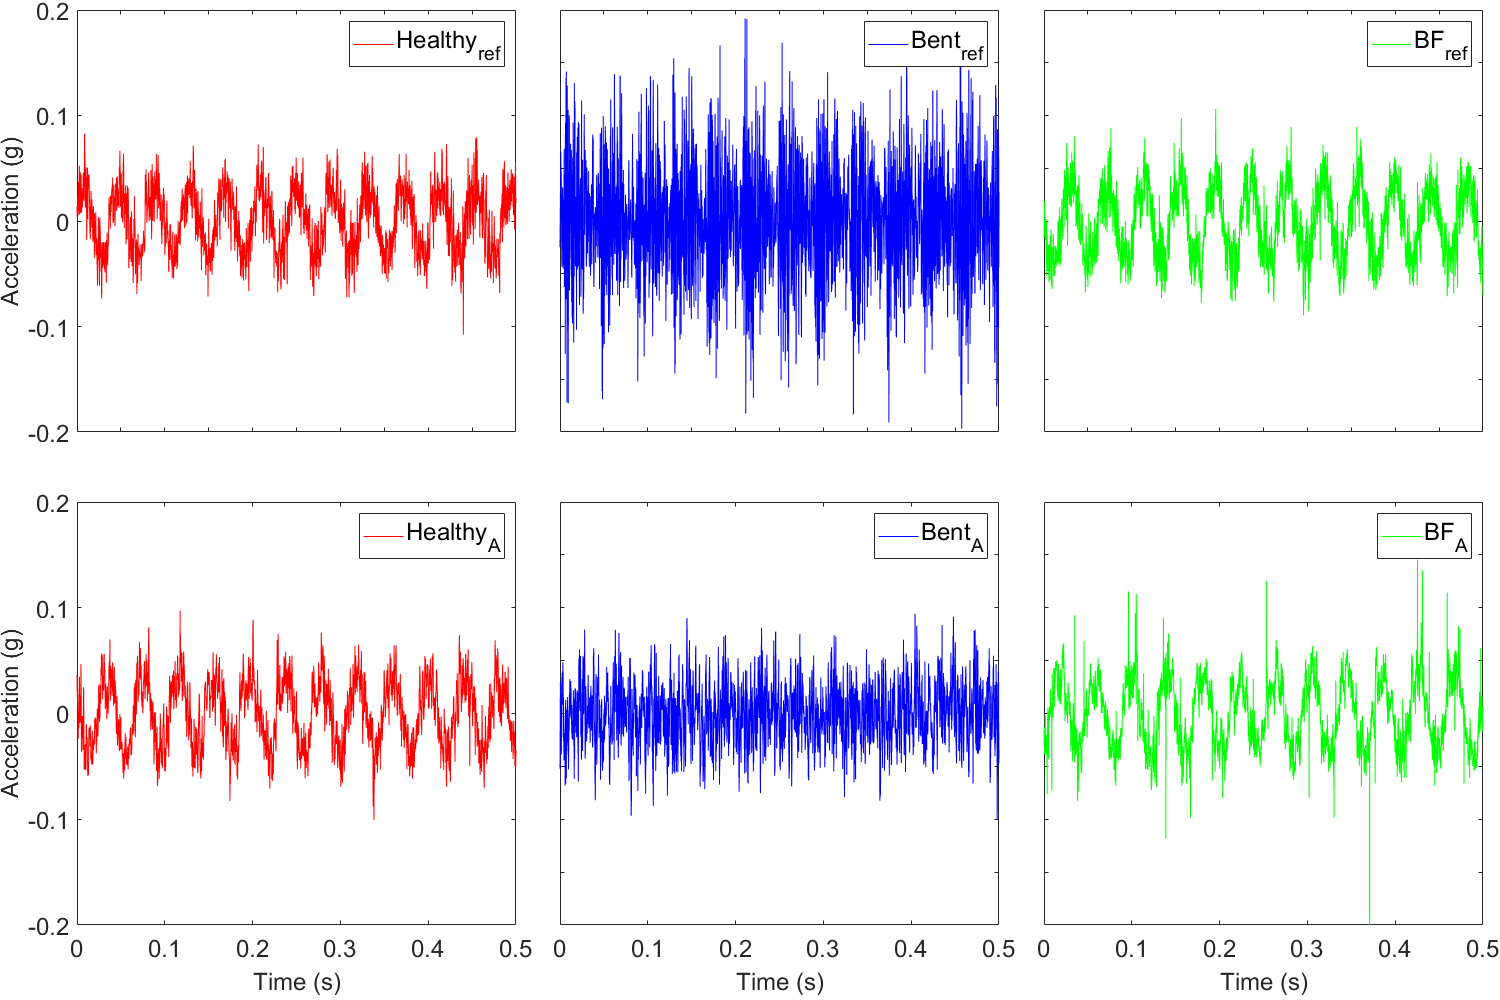
\includegraphics[width=\linewidth]{SensorTest_T.png}
    \caption{Time domain measured by reference and MEMS A sensor for different conditions}
    \label{fig:SensorTest_T}
\end{figure}

The frequency domain provides further evidence that MEMS A performs similarly to the \textit{ref} sensor (Fig \ref{fig:SensorTest_F}).
The spectrum for all three conditions is very similar between the sensors.
Interestingly, MEMS A also performs well above its frequency range of 400 Hz, which was not seen in basic testing.
This is indicated by noticeable peaks in the bent condition spectrum above 400 Hz, although there is a loss of accuracy compared to \textit{ref}.
The bent spectrum also shows noise at around 2 kHz for \textit{ref} and 2.6 kHz for MEMS A.
While this is well above the frequency range of MEMS A, the sampling rate is much higher.
It is possible that the peak seen for \textit{ref} is a result of aliasing and should actually be located closer to 2.6 kHz.
However, this cannot be validated without further testing of \textit{ref}, which is not the focus of this project.
The similarity of the results suggests that MEMS A will also be effective for classifying the condition of the CML.
\par

\begin{figure}
    \centering
    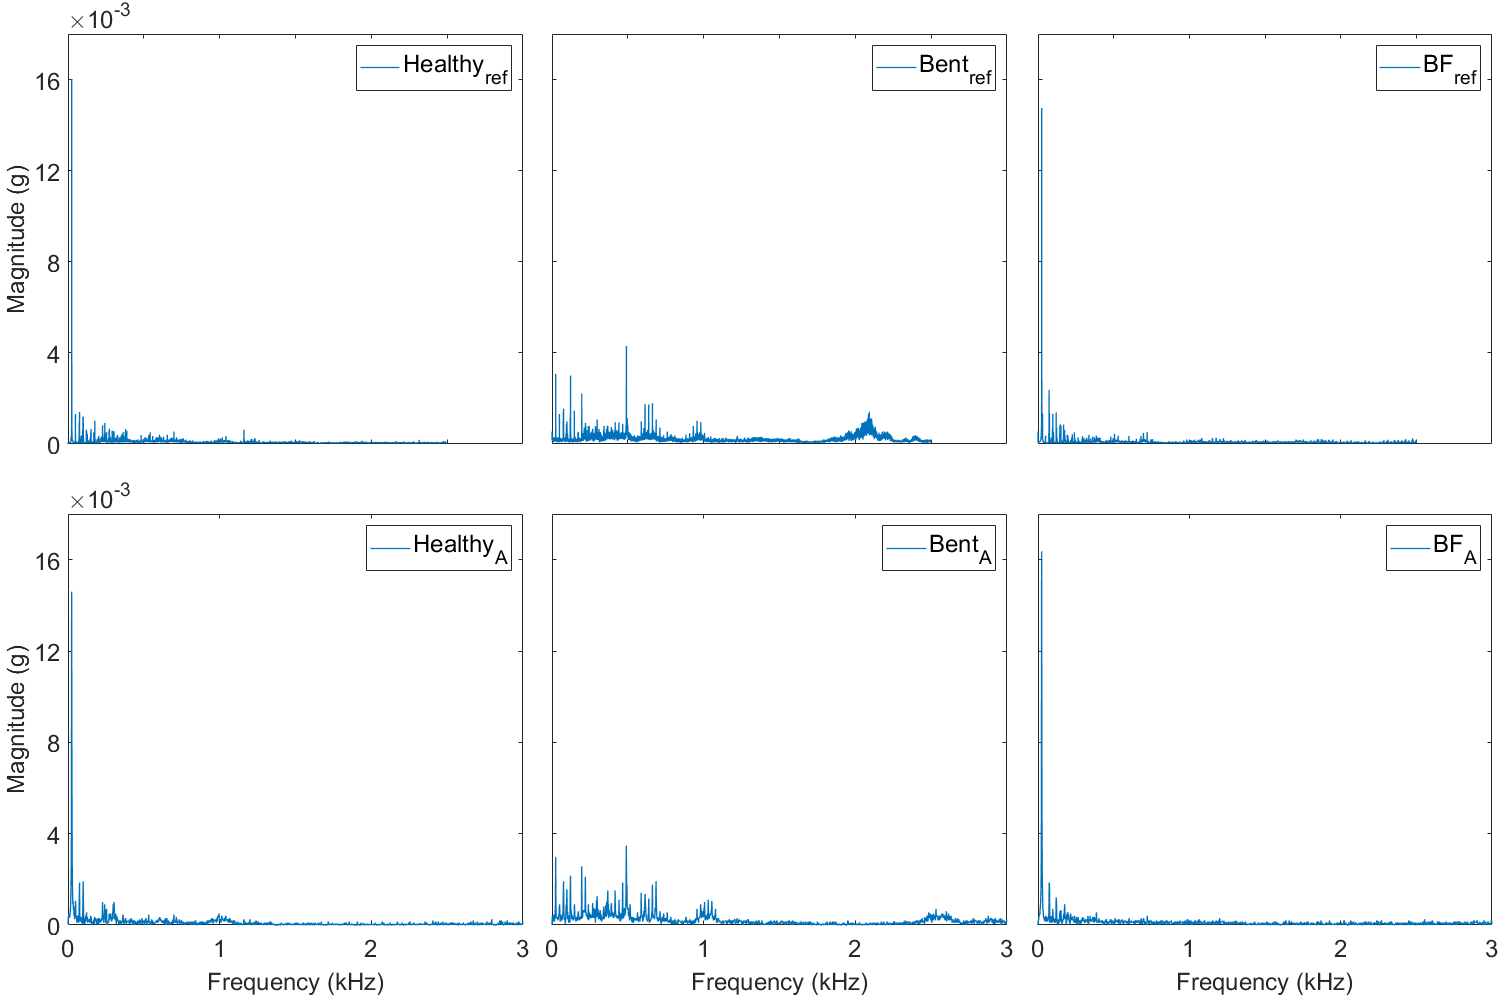
\includegraphics[width=\linewidth]{SensorTest_F.png}
    \caption{Frequency domain measured by reference and MEMS A sensor for different conditions}
    \label{fig:SensorTest_F}
\end{figure}

Extracting statistics from the frequency spectrum shows that the bent condition is easily identifiable for both sensors (Fig \ref{fig:SensorTest_Stats}).
As seen in the initial tests of the CML, the maximum value drops significantly.
The healthy and bearing fault tests are much closer, although the individual readings remain tightly grouped, particularly for MEMS A.
The sensors occupy a similar area of the state space, while not completely overlapping, and correspond well with each other.
One peculiarity is that the bearing fault shows a lower maximum value than the healthy condition for \textit{ref} and a higher value for MEMS A.
Importantly, however, there is a clear difference between the three conditions tested.
\par

\begin{figure}
    \centering
    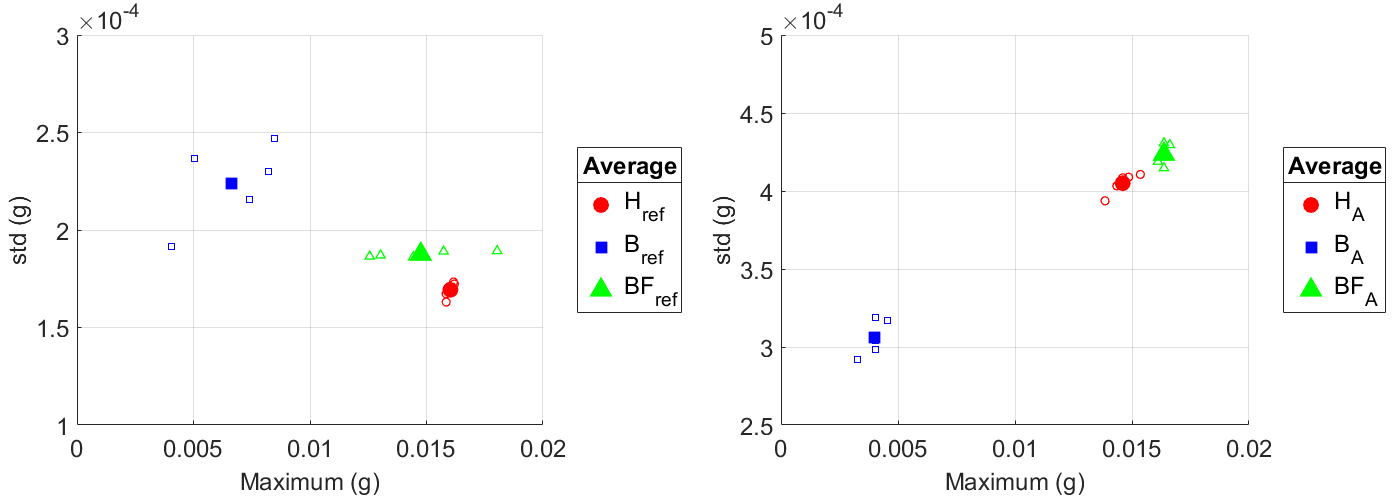
\includegraphics[width=\linewidth]{SensorTest_Stats.png}
    \caption{Comparison of statistics from reference and MEMS A sensors}
    \label{fig:SensorTest_Stats}
\end{figure}

Finally, statistics from the time domain are plotted on the ISO bearing fault severity chart (Fig \ref{fig:SensorTest_ISO}).
There are clear differences between the performance of the sensors, with MEMS A providing more accurate diagnsosis.
The \textit{ref} values suggest that all three conditions fall within the `Normal' boundaries.
Healthy and bearing fault conditions are very close together and the main distinction, as in the frequency domain, is between those two conditions and the bent condition.
MEMS A, on the other hand, shows the healthy and bent conditions very close together, while the bearing fault data falls into the `Alert' range.
It can be seen that the RMS values for all three conditions are similar, but the maximum value is much higher for the bearing fault condition.
This is a result of impulses caused by the bearing fault.
Therefore, the bearing fault severity chart provides a good method for the embedded CMS to distinguish the bearing fault condition, and MEMS A provides accurate information and diagnosis.

\begin{figure}
    \centering
    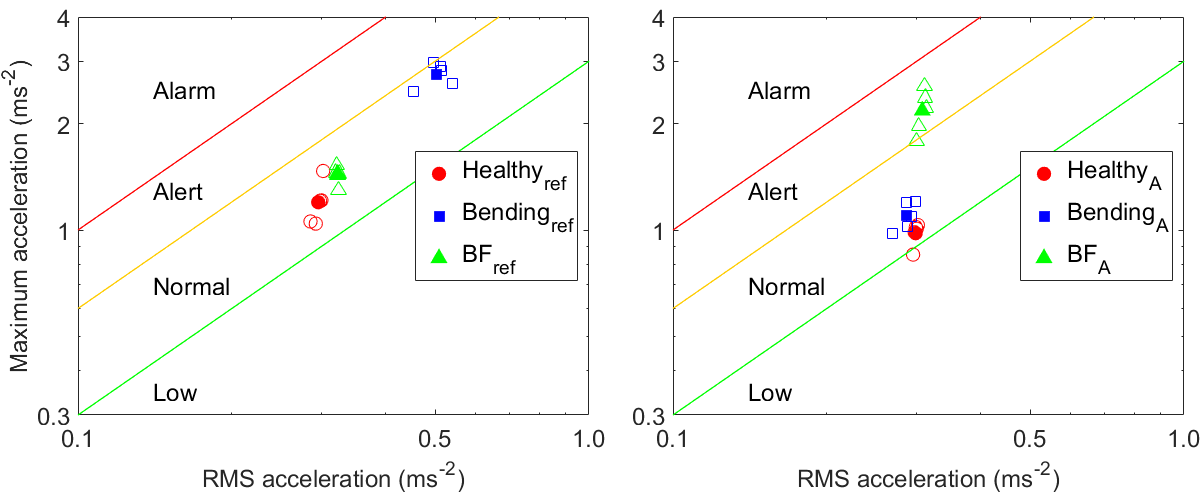
\includegraphics[width=\linewidth]{SensorTest_ISO_Bearing.png}
    \caption{Comparison of statistics from reference and MEMS A sensors against ISO bearing fault severity chart}
    \label{fig:SensorTest_ISO}
\end{figure}

\section{MCSA}

As there is no MCSA implemented on the CML, it is not possible to directly compare the results of any of the following MCSA tests to a data which is known to be accurate.
Testing was conducted with this in mind and an effort to define what the limits of MCSA are for the CML and the embedded CMS.

\subsection{Phases}

Firstly, it was prudent to verify that all three phases powering the motor were working similarly.
This should be the case in a healthy motor, but deviations could be caused by faults in either the motor or power supply \cite{MCSA_Review_Benbouzid}.
As previously noted, the exact condition of the condition monitoring lab is not known \cite{CMlab}.
Both CTs measured the motor in a healthy condition five times on each phase.
The average RMS value in the time domain of the five samples was calculated.
The theoretical sensitivity was used to convert the sensor output to SI units.
The measured sensitivity calculated previously could not be guaranteed to hold in the new conditions of the nCATS laboratory and being close to a power supply with a large heat sink.
A sampling frequency of 4096 Hz was used as the supply frequency of the phases was expected to be around 50 Hz.
\par

The results, shown in Table \ref{tab:current_phase}, indicate that there is not a significant difference in current consumption across the phases.
As before, CT2 shows lower current values than CT1.
The range of current values is very small compared to the range of CT2, so the effective resolution of the sensor is diminished.
All of the values are well within the current limit of 0.70 A specified in the motor datasheet \cite{CMlab_motor}.
Future tests and condition monitoring implementations can use any of the phases for MCSA on the CML.

\begin{table}\centering
    \begin{tabularx}{\textwidth}{@{}*{1}{>{\centering\arraybackslash}X}l*{3}{>{\centering\arraybackslash}X}@{}}\toprule
    \textbf{Sensor} &  \phantom{a} & \multicolumn{3}{c}{\textbf{RMS Current (A)}} \\
    \cmidrule{3-5}
    && Phase 1 & Phase 2 & Phase 3\\
    \midrule
    \textbf{CT1} & & 0.297 & 0.296 & 0.293 \\
    \textbf{CT2} & & 0.248 & 0.252 & 0.263 \\
    \bottomrule
    \end{tabularx}
\caption{RMS current of motor phases during healthy operation}
\label{tab:current_phase}
\end{table}

\subsection{Condition Monitoring}

\begin{figure}
    \centering
    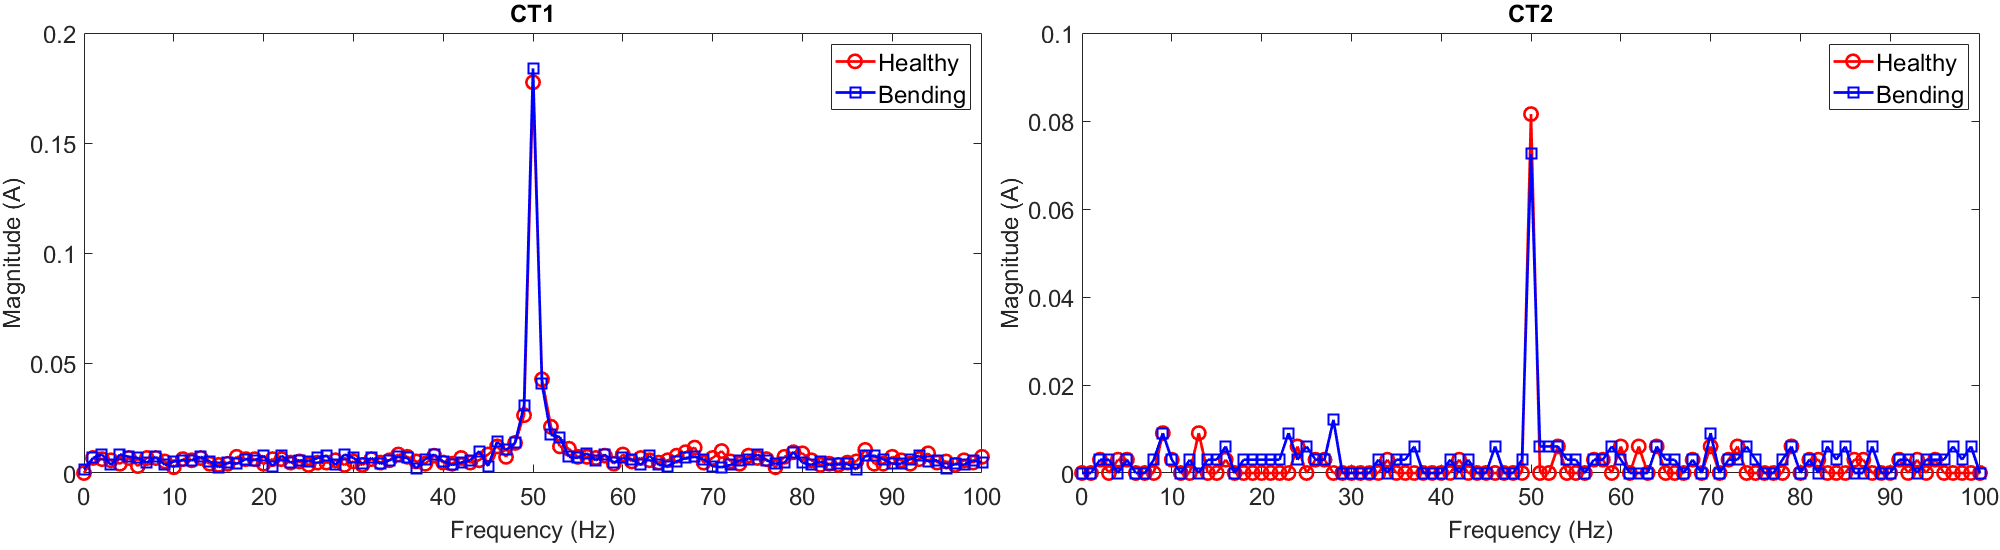
\includegraphics[width=\linewidth]{Current_Test.png}
    \caption{Frequency spectrum of CTs in different conditions}
    \label{fig:Current_Test}
\end{figure}

Next, the CTs were evaluated for their ability to discern between different conditions of the motor.
MCSA can be a powerful technique for diagnosing issues with electrical components \cite{MCSA_Review_Benbouzid}.
However, it should also provide information about the mechanical faults which can be easily tested on the CML.
\par

The CML was tested in the healthy and bending conditions.
The frequency spectrum calculated on board was taken for five samples in each condition.
Averaging of the frequency spectrum from the samples was performed offline to remove noise and allow for a clear distinction between the conditions.
If the bending condition can be detected, it may appear as a heightened value at the suplly frequency as a result of the motor load increasing from increased resistance acting on the bent shaft.
Sampling frequency of 4096 Hz was used.
\par

Both CTs showed very similar frequency spectrums for the healthy and bending condition (Fig \ref{fig:Current_Test}).
Due to its increased sensitivity, CT1 is able to more accurately define the spectrum, reinforcing the similarity between conditions.
Frequencies above 100 Hz are not shown as there were no discernible peaks found in the test data.
The peak of the spectrum has a diminished value in CT2 compared to CT1, given the approximate ration in RMS values seen earlier.
This is due to the increased effect of noise for the sensor with a lower sensitivity.
This noise can also be seen more clearly in the CT2 spectrum.
\par

Given the result of this test and the difficulty in changing bearings on the CML, it was decided not to perform a test for detection of bearing faults using MCSA.
Therefore, MCSA will not be included as a direct input for condition monitoring in the final system design.
In the future, MCSA should be investigated further on the CML for its ability to detect electrical faults.
In the meantime, it can still be used to provide useful information for marine pumps.



\subsection{Speeds}

\begin{figure}
    \centering
    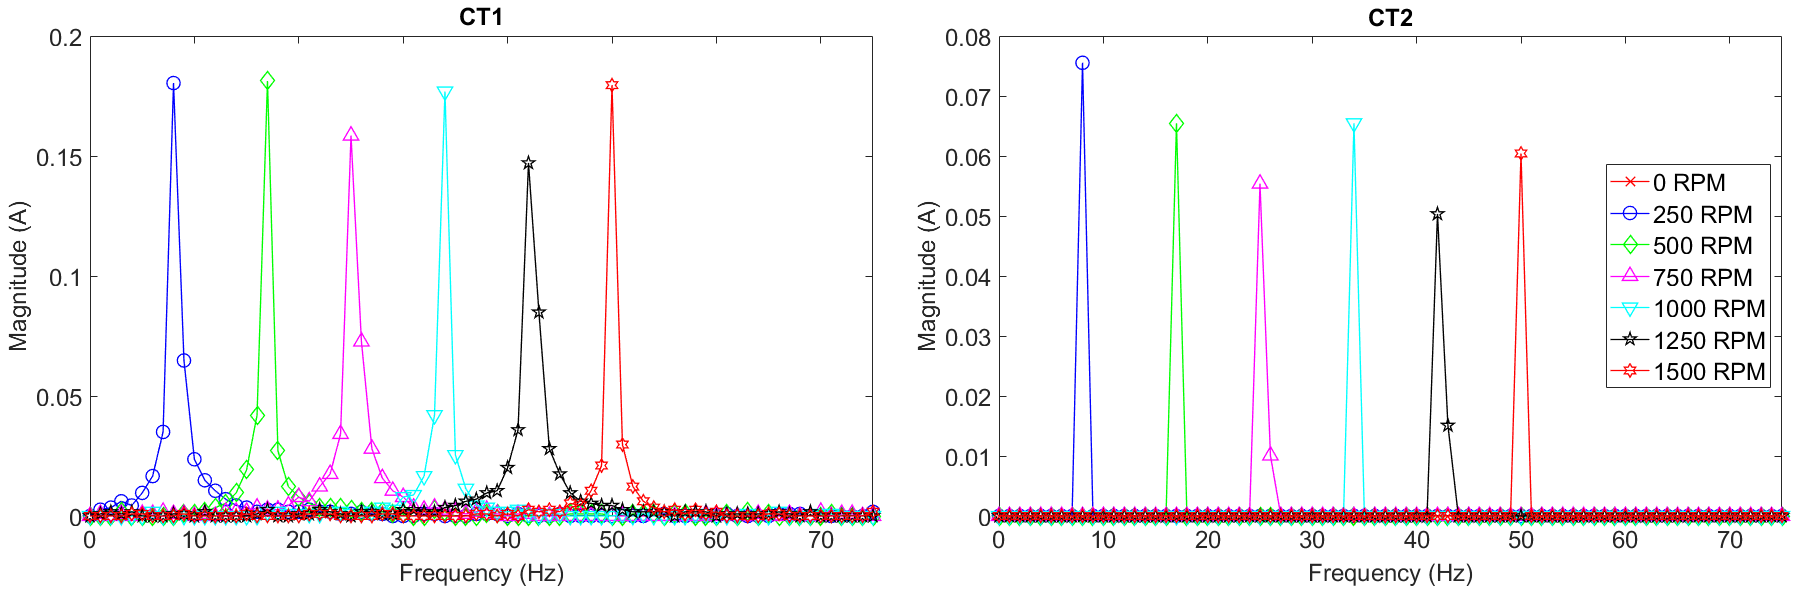
\includegraphics[width=\linewidth]{Current_Speeds.png}
    \caption{Frequency spectrum of stator current measured by current transducers at various motor speeds (legend shared by graphs)}
    \label{fig:Current_Speeds}
\end{figure}

As condition monitoring on ships is currently very poor, even simple information can be of use \cite{CBM_lr}.
This can be as simple as runtime of the motor, which Lloyd's Register understand is not recorded in many instances.
Fortunately, MCSA is well prepared to monitor running time and speed of the motor, as the motor can only run with a large amount of current which will be detected.
With no significant peaks in the frequency spectrum other than supply frequency, MCSA can reliably detect running speed.
This cannot be relied upon as readily with vibration analysis, as there are other significant peaks and the rotor frequency cannot be guaranteed to be the largest, making detection of rotor speed more difficult.
\par

To test the CTs for this purpose, three samples were taken at each speed available on the CML - multiples of 250 RPM from 0 to 1500 RPM.
The frequency spectrum calculated on board was recorded and averaged across the samples.
Sampling frequency of 4096 Hz was used.
\par

Both CTs showed the ability to reliably detect discern the peak and therefore calculate the running speed of the motor (Fig \ref{fig:Current_Speeds}).
Note that although it is included in the results graph, the frequency spectrum of the 0 RPM test is not significant, sugggesting that there is not a lot of noise in the stator current of the CML.
The frequency range shown is limited as there is no significant information in the higher frequencies.
\par

The sampling frequency and sample size limit resolution to 1 Hz, or 60 RPM.
This is reasonable for the CML as it has been designed to only operate at multiples of 250 RPM.
Maintaining a higher sampling frequency allows detection of faults which may be relevant in the future.
However, the requirements of the embedded CMS are dependent on the system being monitored and it may be necessary to increase the resolution if more precise rotor speed information is needed.
With current hardware, the sampling frequency would have to be lowered.

\section{Evaluation}

While it is clear that MCSA offers limited information about machine condition for this CML and the conditions which can be tested, it will provide value to the system.
By using stator current to monitor motor speed, runtime can be measured, providing useful information to users.
Moreover, vibration analysis can then be selectively performed when the motor speed is known to be at the same speed as during testing.
This will help to prevent misdiagnosis due to varying motor speed.
CT1 showed clearer signals and has a higher effective resolution for this CML due to its smaller current range.
CT1 will be used in the embedded CMS.
\par

As was found previously, vibration analysis offers good diagnosis capabilities for the CML.
Unexpectedly, MEMS A sensor showed the best correlation with the existing sensor out of the available MEMS sensors.
It also showed a superior ability over the existing sensor to diagnose faults.
Statistics from the frequency domain provide good diagnosis for the bent condition.
The bearing fault severity chart provides a clearer diagnosis of bearing faults.
Both the time domain and frequency domain should be analysed in the embedded CMS.
MEMS A will be used and can be expected to provide accurate information.